\section{CAnalytics Features}\label{canalytics-features}

\begin{figure}
\centering
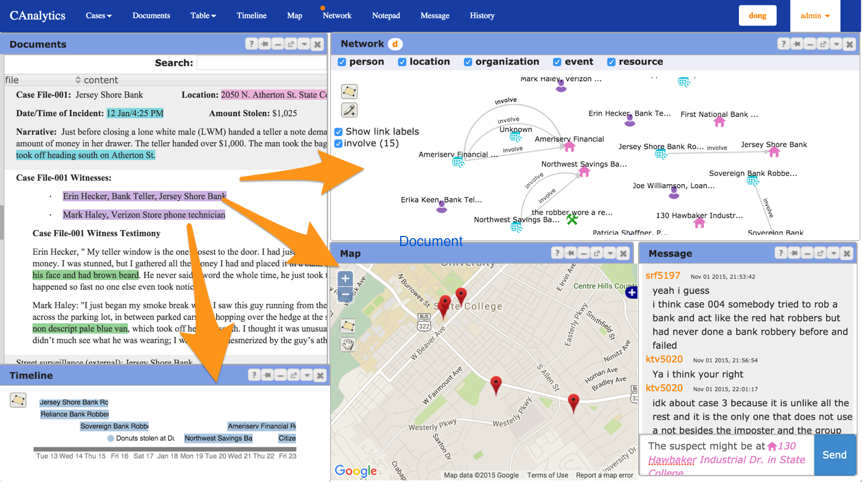
\includegraphics[width=\columnwidth]{03-System/img/interface.png}
\caption{CAnalytics user interface \label{fig:interface}}
\end{figure}

CAnalytics is a web application that aims to provide an integrated workspace
environment wherein teams of analysts identify, visualize, integrate, and assess
facts from multiple sources. The interface is shown in Figure~\ref{fig:interface}. The design is
informed by our cognitive task analysis described beforehand. The system evolved over time. We tagged it as two versions, corresponding to the two classroom studies I have done. Most of the features are available in both v1 and v2, unless noted separately. in v2 we added a couple of new features focusing on hypothesis development, which we will discuss below. 

A use case of applying CAnalytics to an intelligence analysis project: \url{https://youtu.be/2eE92My09Yo}.
A demo of real-time view sharing is available at \url{https://youtu.be/Giz675rMIlE}.And a demo of collaborative hypothesis development is available at \url{https://youtu.be/pHqOukeg2KA}.


\subsection{An integrated workspace: annotation, visualization, and hypothesis}

The CAnalytics workspace is conceptually composed of three functionalities:
annotation for data modeling, visualization for data analysis, and hypothesis
for hypothesis development. To make it an integrated environment, these functionalities share a
consistent interface and data pool, and can communicate to each other in the
same protocol. Each function resides in a self-contained floating window with a title in the top left, a set of functional buttons (help, fixed position, minimize window, maximize window, collapse window, and close window). Users can close a window when that functionality is not needed at the time of analysis to save screen space.

CAnalytics supports evidence annotation in the document view. The
document view displays the text file each analyst receives. When a user selects and highlights snippets of information, a little icon pops up suggesting the text can be annotated. Clicking the icon brings up the annotation editor (shown in Figure~\ref{fig:annotation-editor}). The selected text is used by default as the name of the annotated entity but can be modified by the user. The analyst can then mark the object as one of the following types: person, location, event, resource, organization, and a relationship. These entity types are reported to be the most frequently used by the Red Hat Lab and Colonel Jake Graham . 

Annotations are ``semantic'', meaning
that users are not only highlighting plain text, they are also creating
meaningful, structured data objects with attributes. For example, users can add
such information as gender, job to a person entity. Users can also
make reference to other entities; for example, users can name people who were
involved in an event. Utilities are provided to assist in such input. Figure~\ref{fig:annotation-location} shows the editor of location annotation. A place name-based search utility is provided to help find the place and geographic coordinates as users type. The location entity is then added to the right place in the map automatically.

\begin{figure}
	\centering
	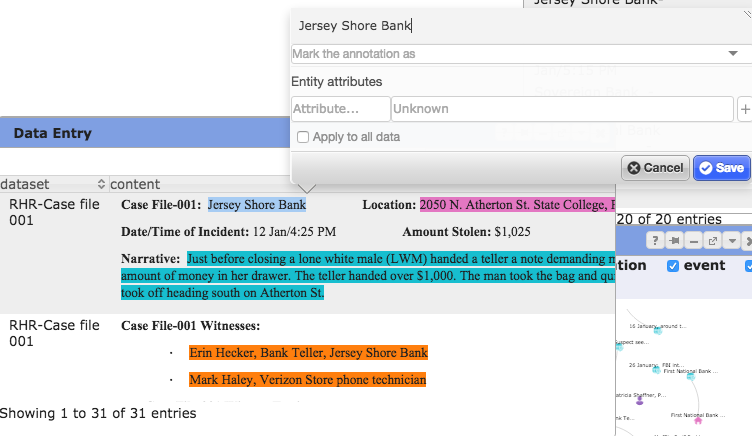
\includegraphics[width=\columnwidth]{03-System/img/annotation-1.png}
	\caption{Annotation in document view \label{fig:annotation-editor}}
\end{figure}

\begin{figure}
	\centering
	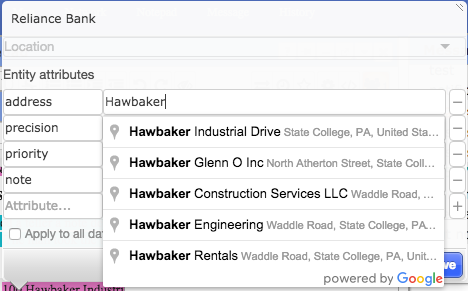
\includegraphics[width=\columnwidth]{03-System/img/annotation-location.png}
	\caption{Utility for location annotation \label{fig:annotation-location}}
\end{figure}

\subsection{Multiple coordinated views of annotated evidence}

CAnalytics supports multiple views for data visualization. Each view provides a means to schematize data, and thus an analytic perspective to understand data:
Timeline organizes data by time, so analysts can do time-sensitive analysis, such as the sequence of events and overlap between events.  The map visualizes evidence by location; with that analysts can do spatial analysis, understanding the proximity of events.  Node-link graph demonstrates the entities and relationships; connected entities are pulled closer by links and form into a cluster. This helps analysts easily decide the role of an entity: if an entity has a lot of connections in a big cluster, it is likely that it plays a leading role in the event. Finally, Table displays entity attributes and allows analysts to examine entities in detail.  

These views are generated automatically from user-created annotations. As shown in Figure~\ref{fig:interface}, when an annotation is created in the
document module, with attribute information about time, location, participants, and their
relationships, a new event is created in the timeline module, a new location is
created in the map module, and new people are created in the node-link graph
module with a typed edge representing relationships among the people (or new
edges are added to existing nodes). Different views are coordinated; that is,
when users do a filter on a piece of information in one view, related
information in other views will be highlighted. Filtering on different
views/schematization provides different analytic strategies; e.g. timeline
offers filtering by time, the map offers filtering by location, and node-link graph
offers filtering by related data objects. Based on the default view of the evidence,
users can continue to schematize it. For example, users can drag the nodes in
the node-link graph to make clusters. Users can also create a relationship in
the graph by drawing a link between two nodes and input relationship attributes.


\subsection{Information sharing and team awareness}

Annotations are immediately shared with collaborators. CAnalytics supports
real-time collaborative editing, similar to Google Tools. Users can open
several concurrent editors to collaboratively edit multiple annotations. Views
are shared together with hypotheses. Team members will then be able to
understand the hypothesis right in that visualization context. They can also
leverage that visualization and continue exploring by reorganizing the view, to
challenge, confirm, or refine the shared hypothesis. In this way, the team is
leveraging each other’s efforts and co-developing hypotheses beyond simply
sharing. CAnalytics has a number of awareness features, including animation of
data change, a notification system, a design we named “tool coordinator”, a
messaging tool, and a history tool. As mentioned before, annotations and data
objects created by collaborators are immediately shared, and updated in the
views. A fade-in and fade-out  animation in the views indicates the creation
and deletion action by collaborators. A notification system sends individual’s
actions to the team, in the form of a text box in the top right corner of the
workspace, keeping the team up to date with collaborator’s actions. To reduce
notification noise, instead of broadcasting whatever actions, we define a set of
rules to determine which actions will be notified. For example, the action that
creates an entity will be notified, but that re-layouts a view will not. Tool
coordinator refers to a small indicator on the tool menu bar, suggesting who is
working on the tool.

A messaging tool enables real time team communication. Chat history is persistent
for traceability. We design a “mention” feature—users can refer to created
entities and relationships in the workspace when they are composing a message.
We believe this will improve communication efficiency because analysts are often
observed to mention critical information entities in a face-to-face discussion.
When the message receiver hovers over the object, attributes of the object shows
up, ensuring that the team is referring to the same thing.

The system maintains a persistent log of time-stamped individual activities. A
history tool presents who did what to which object at when. Together with the
notification system, users who work synchronously can be informed of others’
activity continuously, and be aware of the bigger picture of the team’s activity;
users who work asynchronously will be able to use history to reconstruct
their work status and become aware of changes beyond the point of their last
interaction. Different from awareness features developed in existing systems
which are simply read-only text, the awareness information in our system is
closely integrated with the analytic environment. For example, data objects that
are changed and presented in the history view are clickable links. Users can
hover over to read detailed attributes and click to do a filter on the object.

\subsection{User activity log}

We designed our log schema based upon the work by \cite{Yi2007} and
\cite{Guo2016}. Our log focuses on high level activities that capture the
task the user intends to accomplish rather than their mouse movement. Actions
are categorized under the three top-level activities supported by the system:
data modeling, visual analysis, and hypothesis development. More detailed
actions, their definitions, as well as application-specific actions are shown in
Table~\ref{tab: log}.

\begin{table}
	\caption{Specification of user activities}
	\label{tab: log}
	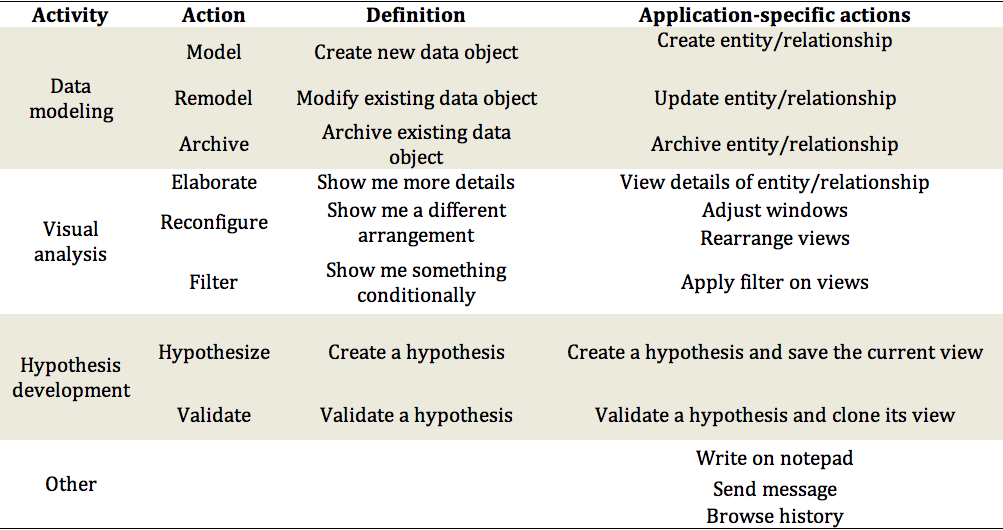
\includegraphics[width=\linewidth]{03-System/img/log_specification.png}
\end{table}


\subsection{Collaborative hypothesis development}\label{feature-hypothesis}

\begin{figure}
	\centering
	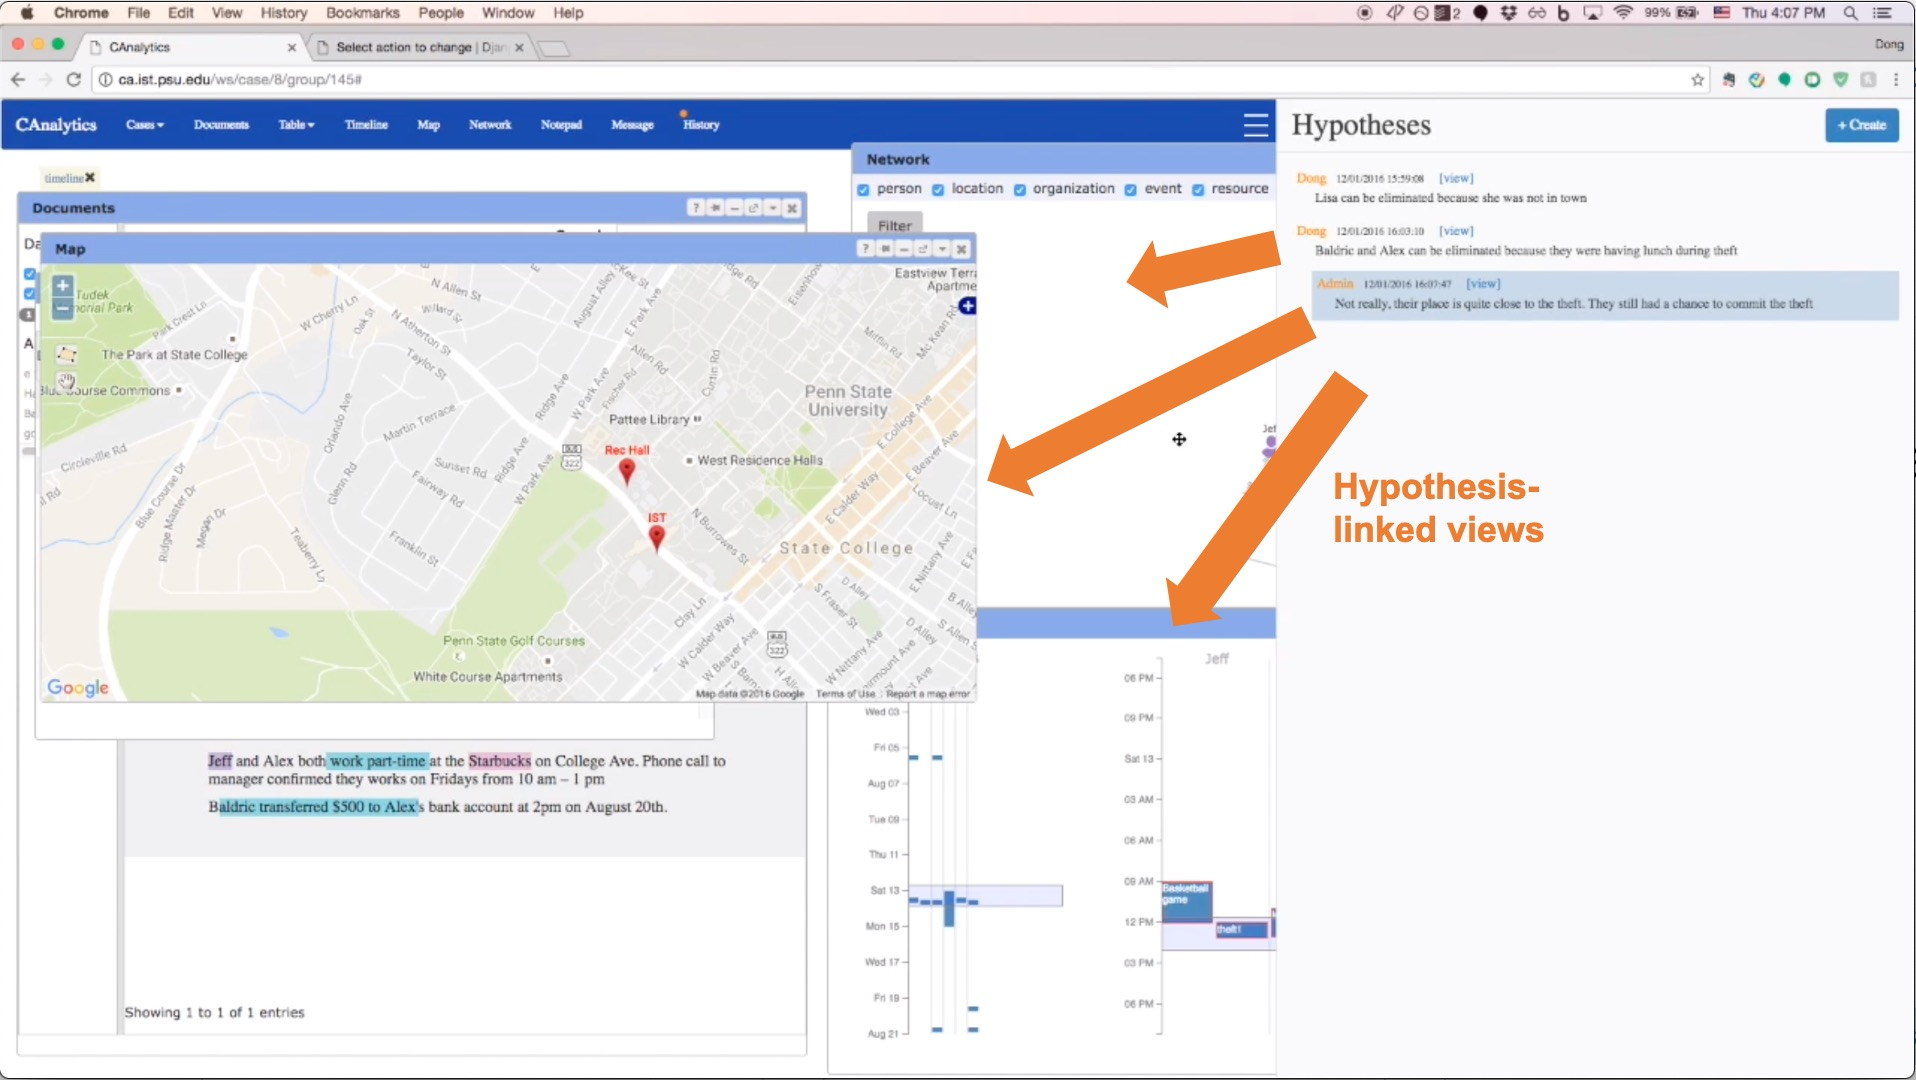
\includegraphics[width=\columnwidth]{03-System/img/hypothesis.jpg}
	\caption{Hypothesis development with linked views \label{fig:hypothesis}}
\end{figure}

All the above features are included in CAnalytics for the first classroom study. In study two, we developed CAnalytics2. A major addition is a structured approach to supporting collaborative hypothesis development. 

In study one with CAnalytics V1, teams put down their hypotheses and notes in a shared note editor. The editor is similar Google Doc, where text is synchronously shared. Hypotheses are shared in plain text, and no structured support is provided. Our first study suggests participants easily lost track of hypothesis development, and it was challenging to re-validate a hypothesis because the context in which it was created was gone. 

In CAnalytics V2, a hypothesis tool is developed as shown in Figure~\ref{fig:hypothesis}. At any time during the process of making annotations or analyzing visualization, analysts can create a hypothesis (with a textual note). In the meantime, the system will automatically record the ad hoc visualization state of all windows, including the data, layout, filtering conditions,etc., and save it together with the hypothesis. The hypothesis is shared with collaborators together with the bound visualization. Teammates who are interested in a specific hypothesis statement can restore the linked visualization. They can then continue to interactively explore the graph from which the statement was derived, either validating or deputing the previous hypothesis, or finding further evidence to propose a new hypothesis. Watch the video demo at  \url{https://youtu.be/pHqOukeg2KA}.